\documentclass[a4paper,UKenglish]{oasics-v2016}
%This is a template for producing OASIcs articles. 
%See oasics-v2016-manual.pdf for further information.
%for A4 paper format use option "a4paper", for US-letter use option "letterpaper"
%for british hyphenation rules use option "UKenglish", for american hyphenation rules use option "USenglish"
% for section-numbered lemmas etc., use "numberwithinsect"
 
\usepackage{microtype}%if unwanted, comment out or use option "draft"
\usepackage[numbers,sort]{natbib}
\usepackage{filecontents}
\usepackage{amssymb}
\usepackage{graphicx}
\usepackage{color, colortbl, xcolor}
\usepackage{algorithm,algpseudocode}
\usepackage{amsmath}
\usepackage{pifont}
\usepackage[font+=scriptsize]{subcaption}
\usepackage[margin=10pt,font=small]{caption}
\usepackage{mwe}
\usepackage{pgfplots}
\usepackage{tikz}
\usepackage{hyperref}% http://ctan.org/pkg/hyperref
\usepackage{filecontents}
\usepackage{epstopdf}
\hypersetup{
	colorlinks,
	linkcolor={red!50!black},
	citecolor={blue!50!black},
	urlcolor={blue!80!black}
}


\definecolor{bblue}{HTML}{4F81BD}
\definecolor{rred}{HTML}{C0504D}
\definecolor{ggreen}{HTML}{9BBB59}
\definecolor{ppurple}{HTML}{9F4C7C}
\definecolor{oorange}{HTML}{FFA500}

%\graphicspath{{./graphics/}}%helpful if your graphic files are in another directory

\bibliographystyle{plainurl}% the recommended bibstyle

% Author macros::begin %%%%%%%%%%%%%%%%%%%%%%%%%%%%%%%%%%%%%%%%%%%%%%%%
\title{Improving the Latency and Throughput of ZooKeeper Atomic Broadcast}
\titlerunning{Improving the Latency and Throughput of ZooKeeper Atomic Broadcast} %optional, in case that the title is too long; the running title should fit into the top page column

%% Please provide for each author the \author and \affil macro, even when authors have the same affiliation, i.e. for each author there needs to be the  \author and \affil macros
\author[1,2]{Ibrahim EL-Sanosi}
\author[2]{Paul Ezhilchelvan}

\affil[1]{Faculty of Information Technology, Sebha University, Sebha, Libya\\
	\texttt{i.elsanosi@sebhau.edu.ly}} 
\authorrunning{I. EL-Sanosi and P. Ezhilchelvan}
\affil[2]{School of Computing, Newcastle University, Newcastle Upon Tyne, UK\\
  \texttt{\{i.s.el-sanosi,paul.ezhilchelvan\}}@ncl.ac.uk}



%School of Computing Science, Newcastle University, Newcastle Upon Tyne, UK,  \email{\{i.s.el-sanosi,paul.ezhilchelvan\}}@ncl.ac.uk}


 %mandatory. First: Use abbreviated first/middle names. Second (only in severe cases): Use first author plus 'et. al.'

\Copyright{Ibrahim EL-Sanosi and Paul Ezhilchelvan}%mandatory, please use full first names. OASIcs license is "CC-BY";  http://creativecommons.org/licenses/by/3.0/
\subjclass{D.2.8 Performance measures, D.4.7 Distributed systems}
%\subjclass{} %Dummy classification -- please refer to \url{http://www.acm.org/about/class/ccs98-html}}% mandatory: Please choose ACM 1998 classifications from http://www.acm.org/about/class/ccs98-html . E.g., cite as "F.1.1 Models of Computation". 
\keywords{% mandatory: Please provide 1-5 keywords
% Author macros::end %%%%%%%%%%%%%%%%%%%%%%%%%%%%%%%%%%%%%%%%%%%%%%%%%
Atomic Broadcast, 
Server Replication, 
Protocol Latency,
Throughput
}
%Editor-only macros:: begin (do not touch as author)%%%%%%%%%%%%%%%%%%%%%%%%%%%%%%%%%%
\EventEditors{John Q. Open and Joan R. Acces}
\EventNoEds{2}
\EventLongTitle{42nd Conference on Very Important Topics (CVIT 2016)}
\EventShortTitle{CVIT 2016}
\EventAcronym{CVIT}
\EventYear{2016}
\EventDate{December 24--27, 2016}
\EventLocation{Little Whinging, United Kingdom}
\EventLogo{}
\SeriesVolume{42}
\ArticleNo{23}
% Editor-only macros::end %%%%%%%%%%%%%%%%%%%%%%%%%%%%%%%%%%%%%%%%%%%%%%%

\begin{document}

\maketitle

\begin{abstract}
	ZooKeeper is a crash-tolerant system that offers fundamental services to 
Internet-scale applications, thereby reducing the development and hosting of the latter.
It consists of $N\geq3$ servers that form a replicated state machine. 
Maintaining these replicas in a mutually consistent state requires executing 
an Atomic Broadcast Protocol,
\emph{Zab}, so that concurrent requests for state changes 
are serialised identically at all replicas before being acted upon.
Thus, ZooKeeper performance for update operations is determined by Zab performance.
We contribute by presenting two easy-to-implement Zab variants, called \emph{ZabAC} and \emph{ZabAA}. 
They are designed to offer small atomic-broadcast latencies and to reduce the processing load on the 
primary node that plays a leading role in Zab. The former improves ZooKeeper performance and the latter enables ZooKeeper
to face more challenging load conditions. 
 \end{abstract}

\section{Introduction}

Apache ZooKeeper \cite{r2} is a high-availability system that is designed to offer several
fundamental services to Internet-scale distributed applications. It is a widely used, industrial-strength
system because it relieves large-scale applications from having to build fundamental services themselves.
Some of the services offered by ZooKeeper include: leader election (used by Apache Hadoop \cite{r28}) and
%\cite{r82}
failure-detection and group membership configuration (by HBase \cite{r82}).

%ZooKeeper is a replicated system being made up of  $N
ZooKeeper is built as a replicated system using $N, N \geq 3$, fail-independent servers.
At most $f = \lfloor\frac{N-1}{2}\rfloor$ of these $N$ servers can crash which means that ZooKeeper can continue to provide uninterrupted services to applications as long as crashed servers are replaced and
at least $f+1$ servers are operative at any given time.


ZooKeeper uses the atomic broadcast protocol, Zab \cite{r2}, to
ensure that ZooKeeper servers' states and its clients are kept in
a consistent state. Zab is typically composed of three to seven machines
which are used for replicating data in order to achieve high availability. In ZooKeeper, one of the nodes has a \emph{leader} role and the rest have
\emph{follower} roles. The leader is responsible for accepting all
incoming state changes (write requests) from the clients and replicating them to
all servers in the ensemble through Zab.

However, many leader-based protocols, including Zab, have problems
associated with overloading, weak writes as well as scalability and bottleneck that occur under write-intensive workloads \cite{r5,r9,r39}.
In Zab, write requests always take longer to process, as they must
go through the Zab and the leader replica, which requires extra tasks
to propagate the requests to all followers since three communication
steps are needed to broadcast a single write request. Consequently, this can
add more latency to the requests and decrease performance.

In this paper, we present two atomic broadcast
protocols, \emph{ZabAC} and  \emph{ZabAA}. ZabAC accomplishes write request
in two-rounds of communication, namely the \emph{proposal} and \emph{acknowledgement-commit} rounds. ZabAC is similar to the Zab protocol, the different is that ZabAC executes a write in two communication steps rather than three. However, ZabAC works only in a three server ensemble. ZabAA can also accomplish a write in two communication steps, and moreover unlike ZabAC, it can utilise any ensemble size, N. We discuss these two approaches in more detail in section \ref{System Model}.

The remainder of the paper is structured as follows. Section \ref{Zookeeper-broadcast-protocol}  describes the design of Zab, an atomic broadcast protocol for the ZooKeeper coordination service. Section \ref{System Model} describes the protocols we developed. Section \ref{Evaluation} provides a thorough performance evaluation of the ZabAC and ZabAA model compared to the existing Zab approach. Section \ref{Related Works} discusses related work. Finally, section \ref{Conclusion} concludes the paper and the outlook for our future research.



\section{ZooKeeper Atomic Broadcast Protocol} \label{Zookeeper-broadcast-protocol}

ZooKeeper is implemented using an ensemble of $N$, $N \geq 3 $, fail-independent and fully-connected servers.
In practice, $N$ is an odd number, typically 3-7 servers \cite{r6}. The following assumptions are made by ZooKeeper.

\subsubsection*{A1 - Crash Tolerance.}
Servers can crash and at least $\frac{N+1}{2}$ servers are operational at any time.
Thus, up to  $f$, $f = \lfloor\frac{N-1}{2}\rfloor$, server crashes are tolerated.

\subsubsection*{A2 - Reliable and Source-Ordered Communication.} \label{A2}
Servers are connected by a reliable communication subsystem in which messages are never lost and are received in the order in which there are sent. More precisely, if a server sends a message $m$ then all operative destinations receive $m$ within some finite time; if a server sends $m_1$ followed by $m_2$, any common destination for $m_1$ and $m_2$ will receive
$m_1$ before $m_2$.

ZooKeeper servers are basically replicas of each other and each maintains a copy of the application state. A Zookeeper client can submit its request or signal an event to any server. If the processing of requests or events from clients does not involve modifying the application state, then the server will respond directly to the client without involving the other servers. 

If however a client request requires modifying the application state, this will be handled by all servers in a mutually consistent manner; that is, it will be identically ordered against any concurrent requests/events received at other servers  before it is processed. Ensuring identical order on concurrent requests and events is accomplished through \emph{Zab}, the ZooKeeper atomic broadcast protocol.

Zab is an asymmetric protocol in its structure: it designates one of the ZooKeeper servers as the \emph{leader} and the rest as \emph{followers}. As with the well-known 2-Phase commit protocol in database transactions \cite{bernstein2009principles}, atomic broadcasting can be initiated only by the leader and followers respond to what they receive. Figure \ref{ZooKeeper Service} depicts how requests and events requiring state modification are handled by ZooKeeper.




%the leader is the server that executes a broadcast by initiating the
%Zab protocol, and any server other than the leader that needs to broadcast
%a message first forwards it to \emph{follower}, receives a state change request from the leader and they also %accept the request. Zab can
%tolerate up to $f$ crash failures out of $2f+1$ servers. The leader
%also needs a quorum of servers, $f+1$, to synchronize its state. The leader
%is connected to each followers through direct \emph{FIFO} channels
%(implemented as TCP streams).
%
%Zab allows clients to connect to any ZooKeeper server, whether the
%server is the leader or a follower. If a client sends a read request
%to a follower, it will be processed locally and the result will be
%sent back to the client, scaling read throughput and fault tolerance
%as servers are added to ZooKeeper's ensemble. There is no need to
%broadcast a read as it does not change the state of the ZooKeeper
%servers. However, if a client sends a write request to a follower,
%it will forward it to the leader to trigger Zab to ensure the write
%applies in at least a quorum of ZooKeeper servers.
%
%Note that as we focus mainly on optimizing Zab protocol, the clients
%role is restricted and only mentions in the time when the writes need
%to be sent to the ZooKeeper server. For ease of explanation, the remainder
%of this paper will denote any API call that does not modify data as
%a \emph{read} and any API call that modifies the server state as a \emph{write}.

\begin{figure}[h]
	\centering
	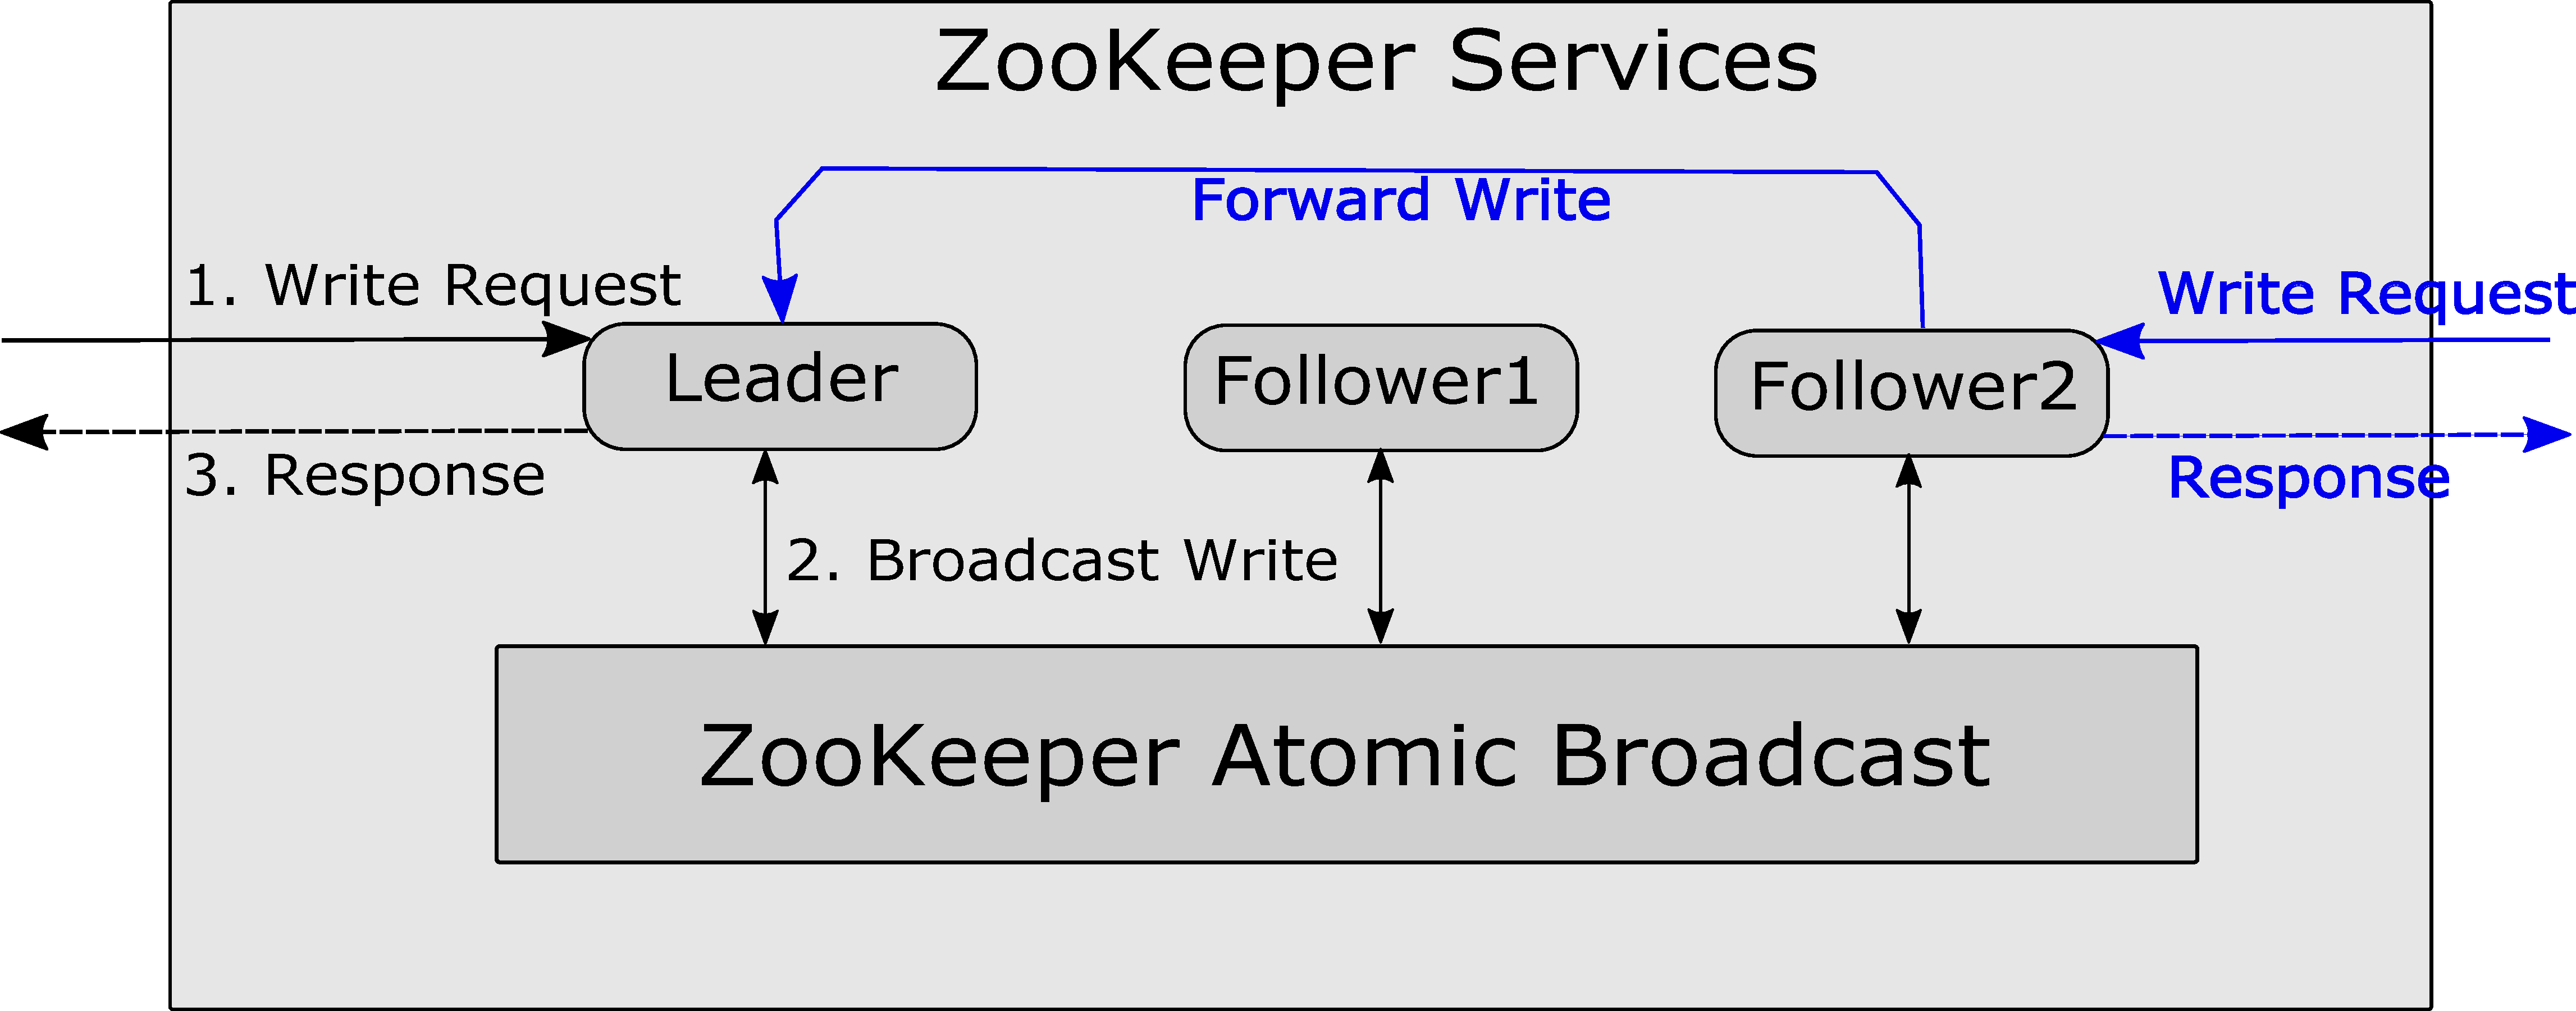
\includegraphics[scale=0.11]{pics/ZKServices.pdf}
	\caption{Write Operations in ZooKeeper}
	\label{ZooKeeper Service}
\end{figure}


%Figure \ref{ZooKeeper Service} shows how ZooKeeper service performs
%write requests sent by clients. Rounds 1-3 are the steps
%executed when a client write request is received, with leader required
%to broadcast the request to the followers. The Figure also shows that all write requests that update ZooKeeper %state are forwarded to  the  leader.

When a follower receives a write request from a client (shown in blue in Figure \ref{ZooKeeper Service}), it forwards it to the leader. Whenever the leader receives a write request that has been forwarded to it by a follower or sent to it directly by a client, it initiates a Zab execution for that request. The execution ensures that the request is delivered to all servers in the same order and only the server that received the request directly from the client returns a response.


\subsection{Zab Protocol}


It consists of the following steps.
\begin{itemize}
	\item L1: Leader initiates \emph{proposal(m)} (state change request) by proposing a sequence number $m.c$ for $m$ and by broadcasting its \emph{proposal(m)} to all processes, including itself;
	\item F1: A follower, on receiving \emph{proposal(m)}, logs $m$
	and then sends an acknowledgement, \emph{ack(m)}, to the leader;
	\item L2: Leader sends \emph{ack(m)} to itself after logging $m$. On receiving \emph{ack(m)}
	from a quorum, it broadcasts \emph{commit(m)} before \emph{commit($m'$: $m'.c = m.c+1$)} is broadcast;
	\item F2: A follower, on receiving \emph{commit(m)}, delivers $m$.
	\item L3: Leader, on receiving \emph{commit(m)} (from itself),  delivers $m$.
\end{itemize}

\subsection{Crash-Tolerance Invariant} \label{Crash-Tolerance Invariant}


Let $\Pi$ be the set of ZooKeeper servers: $\Pi$ =\{$p_{1},p_{2},....,p_{N}$\}. Let \emph{\textbf{Q}} be the set of all majority subsets or \emph{quorums} of $\Pi$: \emph{\textbf{Q}} $ = \{Q : Q\subseteq \Pi \wedge |Q| > f = \lfloor\frac{N-1}{2}\rfloor  \}$.

For example, when $N=3$, \emph{\textbf{Q}} $ = \{ \{p_{1},p_{2}\}, \{p_{2},p_{3}\},\{p_{3},p_{1}\}, \{p_{1},p_{2},p_{3}\}  \} $.

\noindent The \textbf{invariant} is as follows: If any server delivers $m_i$, then all servers in some $Q \in \emph{\textbf{Q}}$ have logged $m_i$ locally.

To see informally that this invariant is a requirement for crash-tolerance provisions, suppose that the leader delivers $m_i$ and then crashes, possibly before broadcasting the commit message for $m_i$. Some quorum of servers, say $Q'$, will elect the new leader and inform it of all messages proposed by leader that crashed. Suppose that the invariant holds and there is a quorum $Q$ of servers that have logged $m_i$. By definition, $Q$ and $Q'$ must intersect. $Q'$ cannot contain the leader that crashed. Thus, $Q$ and $Q'$ must have at least one server in common that is not the crashed leader. That server will instruct the new leader of the existence of $m_i$ and of the need to complete the delivery of $m_i$ by all followers.

%Zab's servers have three modes: \emph{Looking}, \emph{Recovery} and \emph{Broadcast}.

%, then the ZooKeeper
%server needs to synchronises its state with the current leader before
%beginning to serve the clients. Note that we consider the design and
%implementation of the Looking and Recovery phases in ZabAC are
%similar to one use by Zab see \ref{Failure and Recoverys}. Finally, in normal
%execution, when a quorum of servers is up and running, Zab servers consider
%to be in Broadcast mode, where the leader is ready to perform broadcast
%of a client write request. Zab enables write operations to commit
%within three communication steps. It is important to explain the Broadcast
%mode in more detail as it forms the basis of our approach.


\section{Zab Alternatives} \label{System Model}

In this section, we present two protocols that also preserve the crash-tolerance invariant (see section \ref{Crash-Tolerance Invariant}). The first protocol, called \emph{ZabAC}, works only when $N=3$ and the second, called \emph{ZabAA}, is developed for when $N>3$.
%referring to follower send an acknowledgement and commit locally, follower do not need to wait for further an announcement from a leader to commit messages. The second %protocol called \emph{ZabAA}. The ZabAA not just reduce the communication steps but also works with any ensemble.

\subsection{ZabAC}

The design of ZabAC is based on the observation that when $N=3$, the crash-tolerance invariant is satisfied as soon as a follower locally logs the proposal received from the leader. This is because when $N=3$, any two servers constitute a quorum and, given that the leader broadcasts its proposal only after logging it locally, the follower can deliver a proposal as soon as it logs it locally; that is, a follower does not have to wait for an explicit commit message from the leader. The letters \emph{AC} in \emph{ZabAC} stand for the optimisation that followers can acknowledge and commit, without having to wait for an explicit commit message from the leader.

%In this section we introduce a ZabAC protocol, which provides less communication pattens compared to Zab. This protocol was designed for use ensemble size of three-nodes.

%\subsubsection{Processes and Communication.} \label{ZabAC Processes and communication}
%We consider a system $\Pi$ ={$p_{1},p_{2},....,p_{N}$} consists
%of a set of processes that communicate through message passing.
%System makes progress if a quorum of processes $Q$ is up and able
%to send and receive messages. In a quorum of processes, there are
%two roles ZabAC processes can perform according to the protocol: leader
%and follower. Only a leader is able to broadcast, proposing a message
%and sends to all processes. Followers accept leader's messages according to
%the steps of the protocol.

%deleted up to:


%\subsubsection{A4 - Reliable Communication.}
%To meet A3, ZabAC uses reliable UDP and FIFO channel which help to
%deliver proposals in order they have been sent. ZabAC protocol exploits
%using reliable UDP and FIFO channels and thus processes commit locally
%as soon as receiving ACKs from $Q$. Used this way, it is possible
%for processes to decide without waiting for further announcement from
%the leader.This assumption is fundamental part in our proposed protocol, ZabAC.


%In the next section, we describe our technique. We provide more details
%about the design and the implementation of ZabAC protocol.


The key stages of  the ZabAC protocol  are detailed below. Note that $v$ stands for a write request. 
\begin{description}
	\item \textbf{\textbf{\footnotesize 1. Leader Logs and Sends Atomic Broadcast }}- Process a proposal $\langle v,zxid\rangle$ and broadcast it to all processes in $\Pi$.
	\item \textbf{\footnotesize 2. Follower Delivers a Proposal - }Receive, log a
	proposal $\langle v,zxid\rangle$, send an acknowledgement for $\langle zxid\rangle$ to the leader and deliver a proposal $\langle v,zxid\rangle$.
	\item \textbf{\footnotesize 3. Leader Delivers a Proposal - }Receive an acknowledgement
	for $\langle zxid\rangle$, compute a majority of ACK (acknowledgement) and deliver a
	proposal $\langle v,zxid\rangle$.
\end{description}


\subsubsection{ZabAC Implementation Details}

We explore the inner workings of each step of the
ZabAC protocol. We describe each step in the order in which they are
executed by the protocol.\\\\
\noindent \textbf{\small 1. Leader Sends Atomic Broadcast (Proposal Stage)} 


\noindent Prior to commencing the broadcast, a leader places a client's write
operation in its Broadcast Request Pool (BRP), which holds all client
write operations until they are broadcast. When BRP contains operations, a single thread, called \emph{send thread}, is utilised for retrieving
the operations from the BRP and broadcasting them to all processes in $\Pi$.
Operations are retrieved from the BRP in the order in which they were
originally received (FIFO). Upon retrieving an operation, the send
thread creates a proposal message which includes a
tuple $\langle v,zxid\rangle$ that uniquely identifies the broadcast.


Note that, before broadcasting a proposal message, the send thread places
it in a list called \emph{pending} until it receives acknowledgements from a quorum of processes. The pending list contains the proposals. Each proposal waits for a quorum of processes to send acknowledgements to the leader. In parallel, the send thread stores the proposal in \emph{logging} list and periodically logs the list contents in persistent storage for recovery purpose.\\


\noindent \textbf{\small 2. Follower Delivers a Proposal (Acknowledgment and Commit Stage)}

\noindent A follower, on receiving the proposal, first places it in a logging list and periodically logs the list's contents on a disk. After this, the follower must certify that the proposal has the highest zxid that has been received and precedes the last committed zxid. Since the ZabAC uses reliable communication
and FIFO when exchanging messages and the leader sends a proposal in the order according to its zxid, the proposal can always be certified, except when a crash occurs before has been certified the proposal. Once a proposal
is certified, the follower, in parallel, sends an ACK
message to the leader and commits the proposal,
delivering it to the memory. Upon certifying a proposal, the followers deliver the proposal due to receiving ACKs from quorum
of processes: a follower receives one ACK from the leader, piggybacked with
the proposal, and one from itself when it acknowledges the proposal.\\

\noindent \textbf{\small 3. Leader Delivers a Proposal}

\noindent Upon receiving an ACK, the leader delivers the proposal as it receives ACKs from a quorum of processes: it receives one from itself and one from any followers. Note that each process has a \emph{delivered} list which stores all delivered proposals for future read requests by clients. 

\noindent Unlike Zab, ZabAC's leader does not need to send a commit message
to the followers as each follower commits the change locally as soon as it receives ACKs from a quorum of processes. As a
result we save one-third of the communication steps compared to Zab.

Moreover, there are similarities between Zab and ZabAC in the way that proposals are delivered from the perspective of the leader replica. In Zab and ZabAC, a proposal $\langle v,zxid\rangle$ is delivered
as soon as the leader receives an ACK from any follower. However,
ZabAC's leader does not need to process and send a commit message
to $\Pi$. One major difference between Zab and ZabAC is that the followers in ZabAC always deliver a proposal before the leader does, while it is the other way round in Zab. 

%This is explainable
%by the fact that in real environment, if the clients want to have
%latest version for any items, they must connect to the Zab's leader,
%this can add more load to the leader and potential for bottleneck
%to occur. Instead, in ZabAC, the clients can connect to any followers
%to obtain latest version of the item because in ZabAC followers always
%deliver a request before a leader. As a result of clients connect
%to followers, overhead on the leader is reduced. This means that as clients connect to followers
%to read the latest data, the leader become less loaded as compared to Zab's leader.\\

%\noindent  As stated earlier, read requests are serviced from
%the local replica of each Zab process. This allows the service to
%scale linearly as processes are added to the system. Unfortunately, as ZabAC only
%works with three-nodes ensemble, this may not meet the costumer needs,
%scaling read throughput.

%%To circumvent this limitations, we design a new protocol, called \emph{ZabAA}.
%We modify ZabAC in such a way that it can work with any ensemble size, N. We detail our ZabAA protocol in the following section.


\subsection{ZabAA}

ZabAA is developed for any $N$ and as with ZabAC it has been designed so that the leader does not have to broadcast commit messages to its followers. This is achieved by having followers broadcast acknowledgements to every server in the system (\emph{AA} in \emph{ZabAA} stands for \emph{Acknowledge All}). A follower commits a proposal after it (i) receives that proposal from the leader and (ii) knows that at least $f$ followers have acknowledged that proposal. Note that (i) and (ii) ensure that the crash-tolerance invariant is preserved: committing a proposal by a follower occurs only after the leader and at least $f$ followers have logged that proposal locally, and when any subset of $f+1$ servers constitute a quorum in $\Pi$. 

%Unlike ZabAC, we have developed another version of the Zab protocol
%in order to utilise different number of processes $N$ in ensemble
%but exchanging more messages in an acknowledgement stage. The model of ZabAA is very similar to the ZabAC \ref{ZabAC Processes and communication},
%except that upon receiving a proposal message, followers send an
%ACK message (an ACK is sent after proposal persists to the disk) to
%all the processes to which the proposal message is being broadcast see Figure \ref{ZabAA}.
%With this decentralised approach, a process can deliver a proposal
%as soon as it receives ACK messages (which correspond to a given proposal)
%from a majority of processes.


Like ZabAC, ZabAA requires two communication steps: Proposal and Acknowledgement-Commit rounds. Proposal and Commit stages remind unchanged (They are similar to ZabAC implementation). However, the number of acknowledgement messages sent between followers increases quadratically with $N$. Note that ZabAA does not increase the number of acknowledgements that are sent to the leader. ZabAA thus trades-off against higher message overhead for followers. The quadratic increase in follower message overhead may off-set the gain from reduced  follower latencies as $N$ increases. Yet, it is worth investigating ZabAA to study the effect of this trade-off for small values of $N$, particularly for $N=5$ which is the second most typically value (after $N=3$).



\section{Experiments and Performance Evaluation} \label{Evaluation}

In this section, we present a comparative evaluation of Zab, ZabAC and ZabAA. We study different performance metrics: namely latency and throughput.

We used 250 simultaneous clients executed on 10 machines; with each machine operating up to 25 clients. Up to 5 machines were dedicated to run evaluated protocols, typical ZooKeeper installations use 3-7
servers, so 5 is just smaller compared to a typical setting \cite{r2}. All machines in the experiment utilised commodity PCs of 2.80GHz Intel Core i7 CPU and 8GB of RAM,  running Fedora 21 and communicating over 100 Mbps Switched Ethernet.

The evaluated protocols were implemented in Java (JDK 1.8.0) on the top of the JGroups framework; JGroups is a toolkit for reliable communication and it is used to establish a group membership where members can send messages to each other. All messages were transmitted using JGroups' reliable UDP. As well as using a reliable UDP, the JGroups' UNICAST3 protocol is used to provide node-to-node ordering as the default for each message sent. Utilising a UNICAST3 protocol provides FIFO ordering similar to a TCP protocol.

Each request consists of a read or write with 1000 bytes of maximum payload, which represents a typical request size \cite{r2}. In our experiment, 1 million requests were sent. Each client was responsible for sending $\frac{(\frac{10^{6}}{10machines})}{25clients}$ requests. To distribute the load equally on the server protocols, the clients sent the requests to the protocol in a round robin manner. Our benchmark client used the synchronous JGroups client API.

Experiments are run in failure-free scenarios.
Furthermore, servers do not log a proposal message in disk (as ideally required)
but only record the proposal in main-memory.
Thus the performance figures we present here do not include disk write delays, but only
network delays. This kind of evaluations corresponds to the
'Net-Only' category of the evaluations in \cite{r2} where several ways of logging
have been considered. Since Zab and proposed protocols require logging of the proposal message
exactly at the same point in the execution for every broadcast,
ignoring delays due to disk writes cannot invalidate the integrity of
observations made and conclusions drawn from the
performance figures.


Note that the latency is defined here as $t_{1}-t_{0}$ where $t_{0}$ is the time at which a client sends a request to a protocol's server and $t_{1}$ is the time at which the client receives a replay message from the server. So, the final latency is an average of the computed latencies for all clients. We compute the average of $1000000$ such latencies and repeat  the experiment $10$ times for a confidence interval of $95\%$. Throughput is defined as the number of requests made by all servers  per unit time and is computed, like latencies, with a $95\%$ confidence interval. 


\subsection{Zab vs ZabAC}

In this experiment, we deployed Zab and ZabAC in a three-server ensemble since ZabAC works only when $N=3$. Figure \ref{LatencyAC3} shows the latency in milliseconds (ms) of the mixed workload (the ratio of writes to reads) as the percentage of writes was increased. The figure shows that increasing the number of writes has a negative impact on the performance of Zab and ZabAC. The reason the performance is affected is because write requests must go through atomic broadcast, which requires additional processing and adds more latency to requests whereas read requests require the server to only read data from the local replica's state.

 \begin{figure}
	\begin{subfigure}{.5\linewidth}
		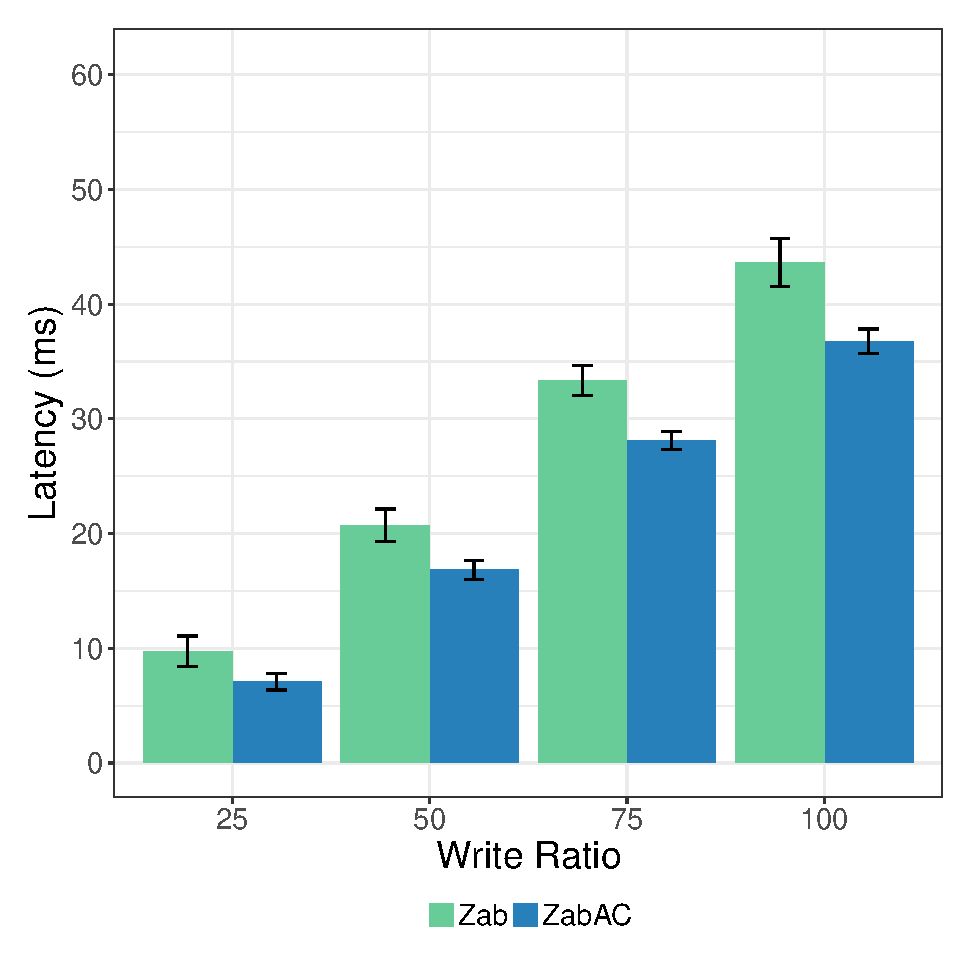
\includegraphics[width=180pt,height=140pt, scale=0.39]{figuress/LN3_AC.eps}
		\caption{Latency comparison}
		\label{LatencyAC3}
	\end{subfigure}		
	\begin{subfigure}{.5\linewidth}
		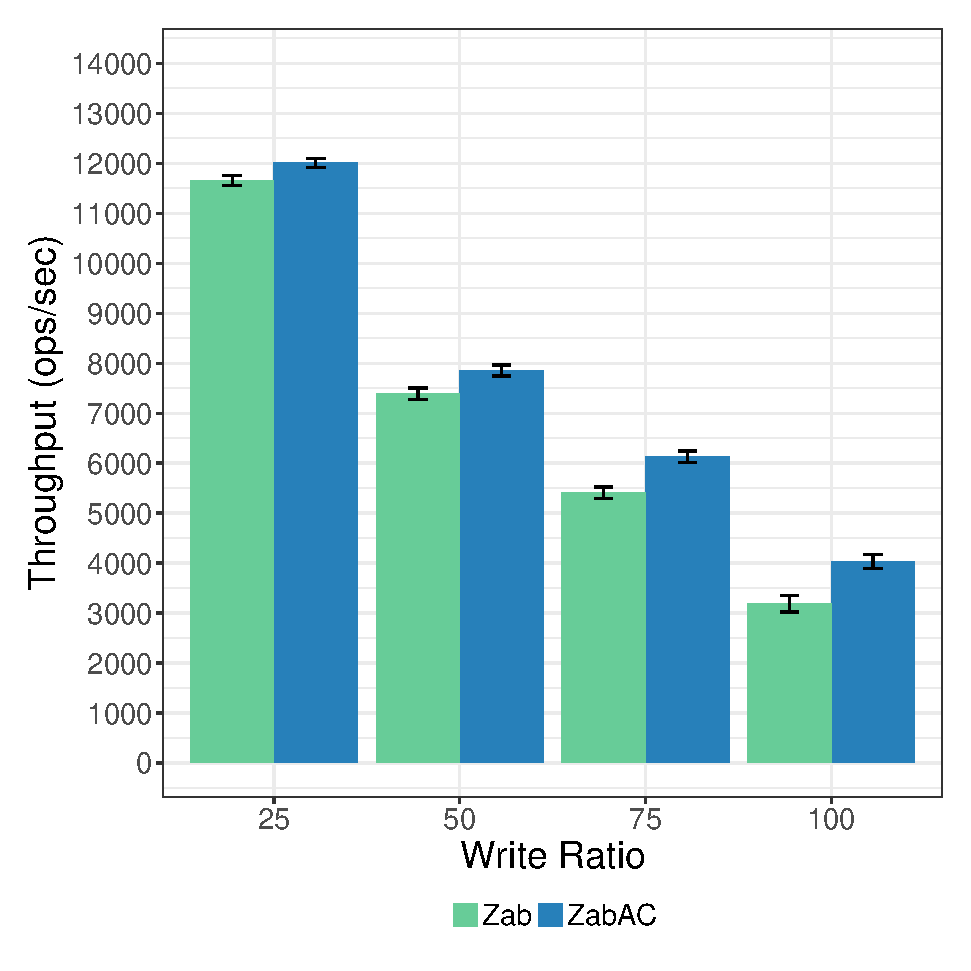
\includegraphics[width=180pt,height=140pt, scale=0.39]{figuress/TN3_AC.eps}
		\caption{Throughput comparison}
		\label{ThroughpuAC3}
	\end{subfigure}		
\caption{Performance comparison, varying the ratio of writes to reads.}
	\label{latency comparison}
\end{figure}


The graph also shows that the latency for ZabAC is lower than for Zab in all writes to reads ratios. For example, with a 100\% writes, ZabAC's latency is approximately 37 ms whereas Zab's latency is 44 ms. This finding was expected because ZabAC has lower overheads as a result of fewer messages being broadcast generally and more specifically because it dispenses with the leader having to send commit messages to its followers.

%With three replicas, our average write latency is 10.5ms. The client then requests to add back four replicas, followed by another write batch. Using our approach write latency is at 11.4ms and jumps to 18.1ms if we stall the pipeline

%\footnote{The average latencies presented in this section are taken over 20 executions of the described experiments.}


%As we scale the number of servers we saturate the network card of the leader which causes the throughput to decrease as the number of servers increases. We can use a broadcast tree or chain replication [7] to broadcast the proposals to avoid this saturation, but our performance is much higher than we need in production, so we have not explored these alternatives.

Figure \ref{ThroughpuAC3} shows a throughput comparison between Zab and ZabAC. Throughout the figure, ZabAC has a higher throughput compared to Zab in all cases, with the maximum difference being 846 operations per second (ops/sec)  (operations size is 1000 bytes) when the number of writes is 100\%. This is due to the fact that in ZabAC there are fewer communication patterns and less network traffic than in Zab. In other words, reducing the number of communication steps results in less computation being performed by the leader, which creates a significant throughput advantage for ZabAC. 

\subsection{Zab vs ZabAA}

In this section, we investigate the effect of ensemble size in Zab and ZabAA. 


Figures \ref{LatencyAAN3} and \ref{LatencyAAN5} show how latency varies according to the size of the ensemble and the workload (the ratio of writes to reads requests). Each figure corresponds to a different ensemble size. We can see that the larger the ensemble size, the higher latency there is in both Zab and ZabAA. This is because the leader needs to synchronize its state with a quorum of replicas, that is, the larger the ensemble size, the longer the leader has to wait before delivering a proposal (for instance, with an ensemble size of three ($N=3$), only two acknowledgements are needed whereas with an ensemble size of five ($N=5$) the leader must wait until it receives an acknowledgement from three replicas). Thus, increasing the ensemble size has an impact on both latency and throughput.


Moreover, each figure shows that latency increases when the workload includes more writes than reads. This could be due to the fact that write requests must go through atomic broadcast and this requires additional processing which, in turn, causes further delay, thus increasing latency.



%	which latency becomes unnoticeable

%	we observe that iSCSI over Gigabit LAN has a relatively lower latency as compared with iSCSI
%The difference becomes larger with the increase of data size
Comparing ZabAA with Zab, we observe that ZabAA experiences lower latency than Zab for all types of workload and ensemble size. Moreover, the difference becomes more significant when the percentage of write requests increases. For example, with 100\% writes and an ensemble size of three, latency is approximately 37 ms for ZabAA and 44 ms for Zab. Likewise, with 100\% writes and an ensemble size of five, latency is approximately 95 ms for ZabAA and 103 ms for Zab. This difference in latency between ZabAA and Zab stems from the fact that in ZabAA only two communication steps are required to deliver a request whereas in Zab three communication stages are needed. 

Unsurprisingly, when the percentage of read requests increases, small differences were found between Zab and ZabAA in term of latency, although ZabAA experiences slightly lower latency than Zab. This small difference in latency could be due to the fact that, as previously stated in section \ref{Zookeeper-broadcast-protocol}, reads are in-memory operations and are serviced from the local replica which means no agreement protocol needs to be run and therefore, latency are decreased and becomes less significant when comparing ZabAA with Zab.   


Figure \ref{ThroughputAAN3} and  \ref{ThroughputAAN5} shows how throughput varies with the number of servers and a mixed workload. The figures indicate that since the leader propagates a proposal to all followers, the throughput must drop as the number of servers increases. Another possible explanation for a decrease in the throughput is that as we scale the number of servers (from three to five), we saturate the network card of the leader. Therefore, the throughput of the evaluated protocols depends on the number of servers connected to the leader as well as write ratio.


Comparing the two protocols, it can be seen that at 100\% writes, ZabAA's throughput is higher than that of Zab, with the maximum difference being relatively significant, approximately 520 ops/sec for $N=3$ and 278 ops/sec for $N=5$. There are two possible explanations for this result. First, ZabAA's leader does not process and broadcast the commit message, unlike in Zab. Second, ZabAA only requires two communication steps to complete write request whereas Zab requires three communication steps. However, the difference in throughput becomes less noticeable as the number of reads increases; the reason being once again that, no additional CPU processing or network load when servicing read requests (in both ZabAA and Zab), which in turn makes the difference between ZabAA and Zab in terms of throughput of less significant. In fact, an increase in the number of reads to writes leads to better overall performance in both protocols. 

One interesting observation that has arisen from this experiment is that the ZabAA protocol has a better performance than Zab in terms of latency and throughput at 100\% write when $N=3$ and $5$. We observe that broadcasting an acknowledgement to all servers in the ensemble does not seem to impair the overall performance, but it might  impact on the performance if $N$ increases to $7$ or more as the number of acknowledgment broadcast increases. 
%it becomes insignificant.
%which latency becomes unnoticeable
%not significantly different



\section{Related Work} \label{Related Works}


Leader based protocols tend to overload the leader %disproportionately (compared to followers)
and several authors	\cite{r5,r9,r39,r37} have sought to remedy this drawback.
S-Paxos \cite{r5} relieves the leader from broadcasting client requests by
separating the roles of request dissemination and request ordering.
Each process directly broadcasts client requests to others %(instead of forwarding to the leader)
and request ordering is done %through Paxos executions
using only request identifiers.
Chain replication \cite{r39} reduces the leader load by distributing the role between two servers called the \textit{head} and the \textit{tail} %. The head is responsible for handling write requests
%and provides $m.c$ for each write which it passes down the chain sequentially until received by the tail.
but involves sequential transmission of message which tends to increase latencies for large $N$.

The benefit of sending an acknowledgement as a broadcast instead of a unicast is explored in the algorithm described in \cite{r41}. More importantly, to our knowledge, although the approach of ZabAA (changing from unicast to broadcast) is relatively simple, no previous study has evaluated it or exposed the trend, particularly in leader and quorum-based protocols. 



\section{Conclusion} \label{Conclusion}

We have presented ZabAC and ZabAA as atomic broadcast protocols
that follow a leader-based approach, similar to Zab. ZabAC and ZabAA guarantee the delivery and order of requests which means that each process has an equal opportunity of having its messages delivered in the same order. ZabAA is an alternative to ZabAC when $N > 3$.

Performance benchmarks showed that ZabAC had low latency and high throughput. Furthermore, by increasing the number of replicas, the ZabAA protocol not only becomes more fault tolerant but also achieves higher throughput and lower latency than the Zab protocol.


Further investigation needs to be accomplished. We plan to evaluate ZabAA using $N=7$ and $9$ to measure latency and throughput. Moreover, our research is currently being carried out to reduce the ZabAA's message overhead by conditioning the sending of acknowledgements on the outcomes of coin tosses.


%We intend to continue with experimental work to better understand the strengths and weaknesses of our the approach. In particular, we currently pursue two directions: one is to make the protocol more agressive regarding the fast deliveries of transactions, the other is the study of the protocol’s behavior in heterogeneous large-scale networks.

\appendix

\section{Source Code}
The source code for the evaluated protocols and the benchmarks are publicly available at https://github.com/ibrahimshbat/JGroups.

\section{Performance Compression for Zab and ZabAA}

\begin{figure*}[h]
	\begin{subfigure}{.5\linewidth}
		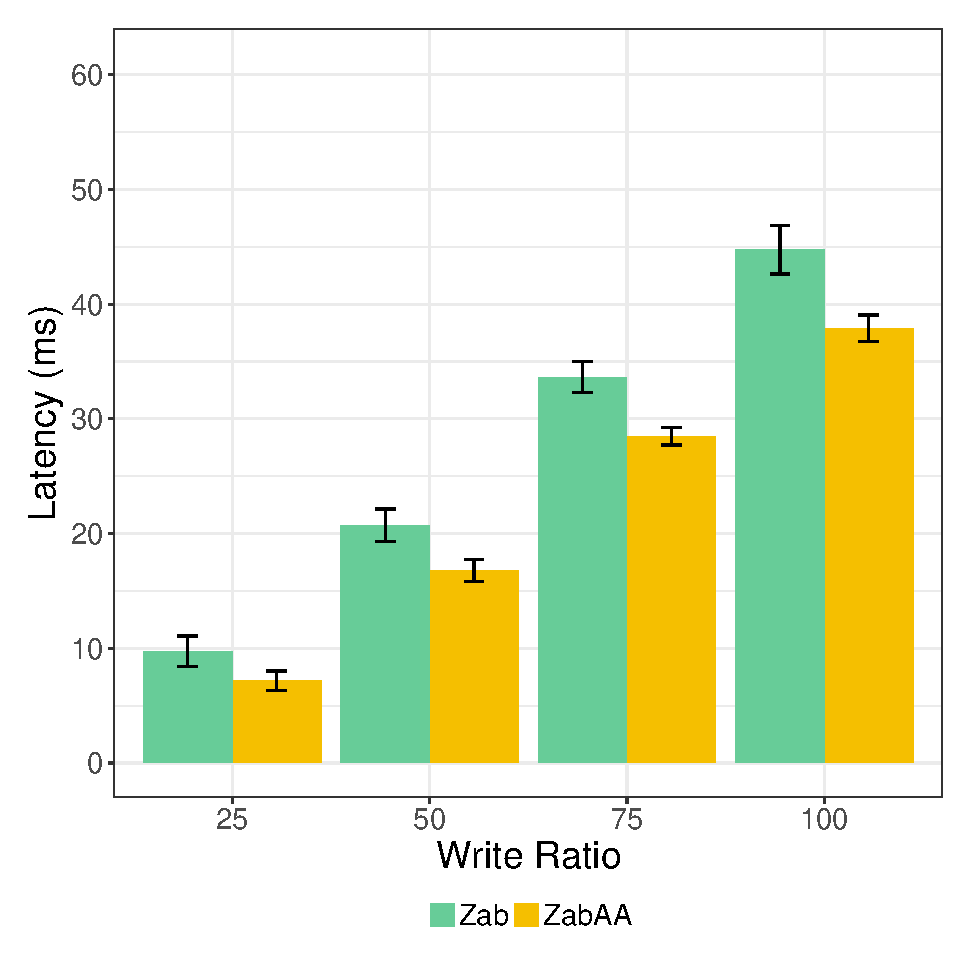
\includegraphics[width=170pt,height=140pt, scale=0.39]{figuress/LN3_AA.eps}
		\caption{Ensemble size $N=3$}
		\label{LatencyAAN3}
	\end{subfigure}		
	\begin{subfigure}{.5\linewidth}
		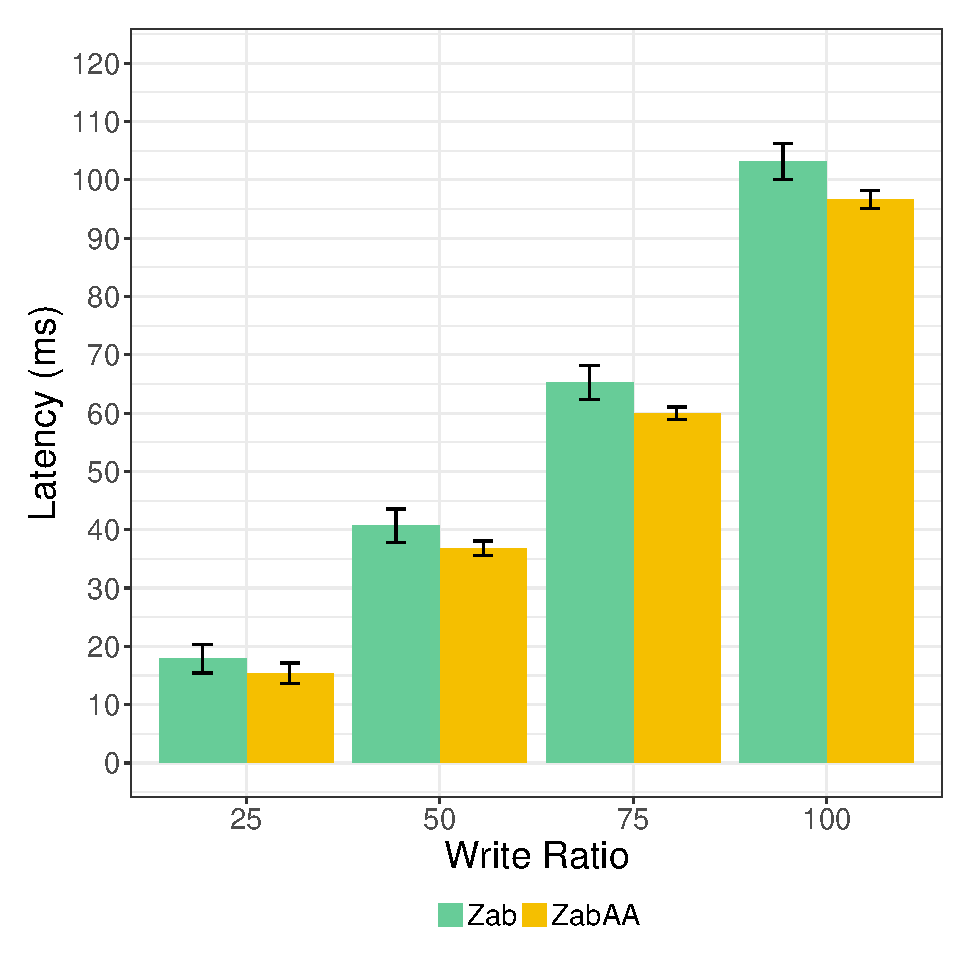
\includegraphics[width=170pt,height=140pt, scale=0.39]{figuress/LN5_AA.eps}
		\caption{Ensemble size $N=5$}
		\label{LatencyAAN5}
	\end{subfigure}		
	\caption{Zab and ZabAA latency comparison, varying the ratio of writes to reads.}
	\label{latency comparisonN3}
\end{figure*}


\begin{figure*}[h]
	\begin{subfigure}{.5\linewidth}
		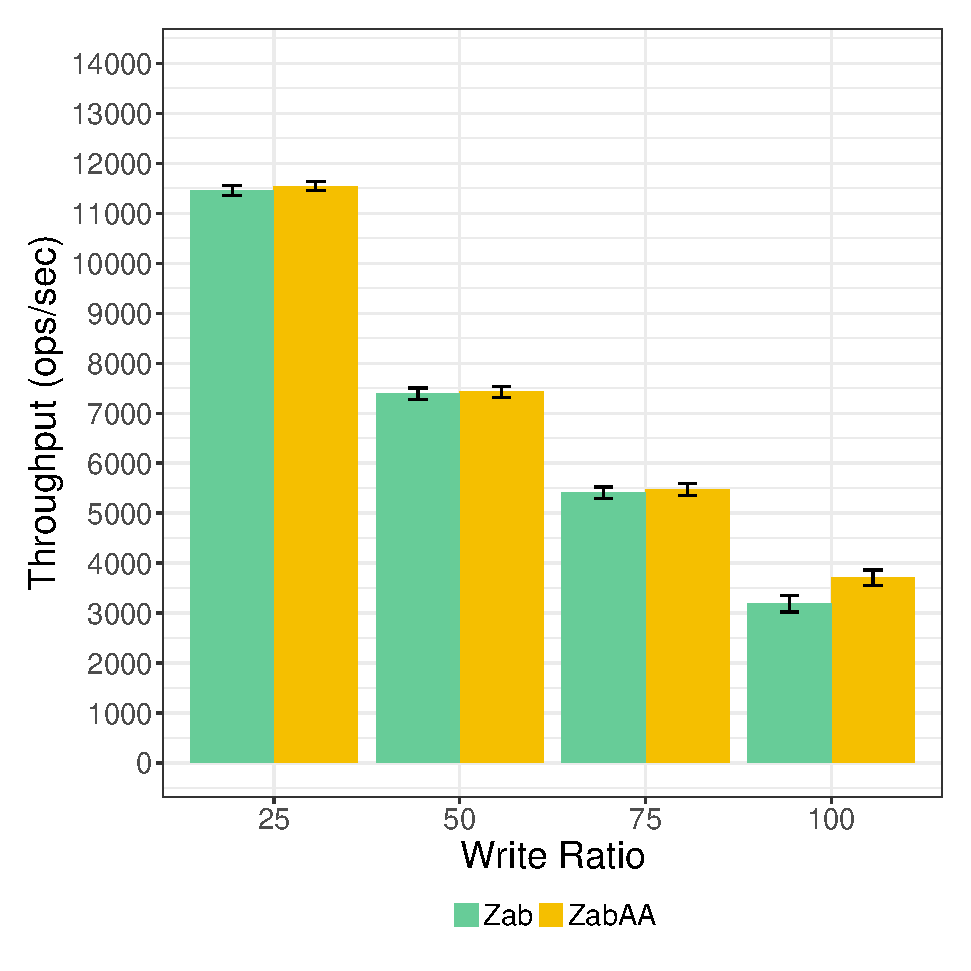
\includegraphics[width=170pt,height=140pt, scale=0.39]{figuress/TN3_AA.eps}
		\caption{Ensemble size $N=3$}
		\label{ThroughputAAN3}
	\end{subfigure}		
	\begin{subfigure}{.5\linewidth}
		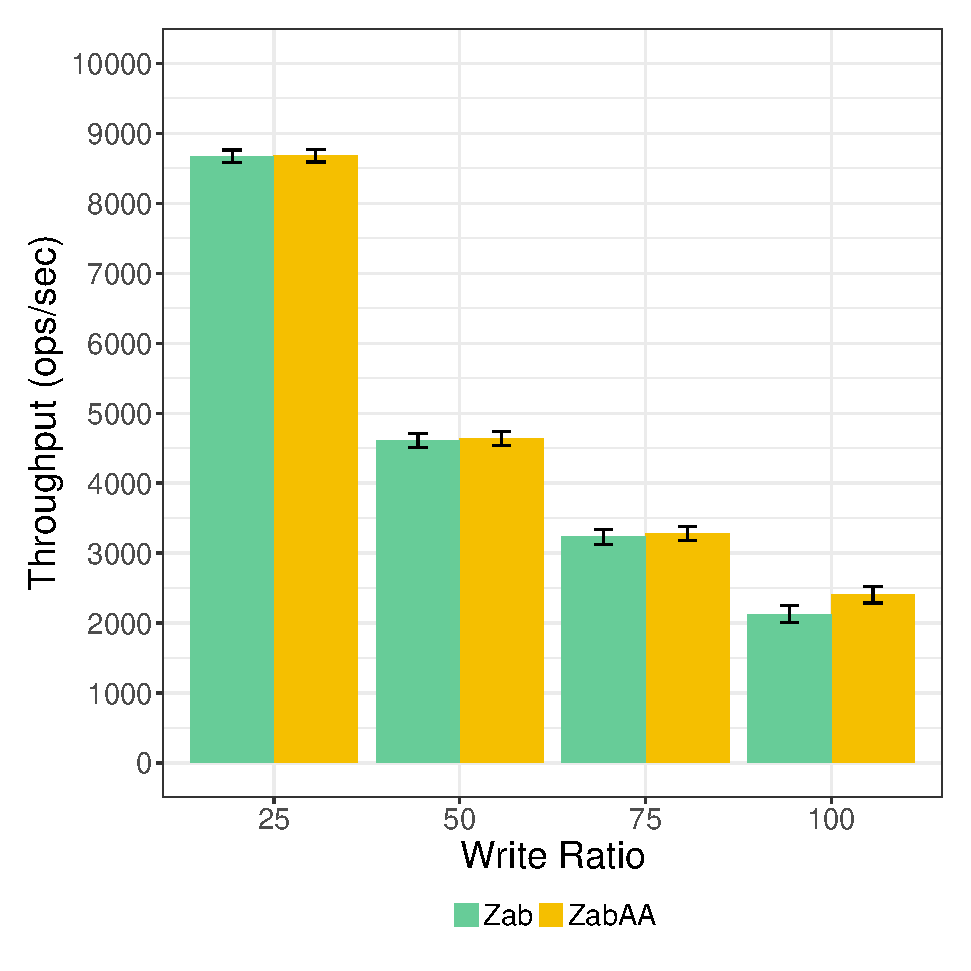
\includegraphics[width=170pt,height=140pt, scale=0.39]{figuress/TN5_AA.eps}
		\caption{Ensemble size $N=5$}
		\label{ThroughputAAN5}
	\end{subfigure}		
	\caption{Zab and ZabAA throughput comparison, varying the ratio of writes to reads.}
	\label{latency comparisonN5}
\end{figure*}

\bibliographystyle{oasics-v2016-sample-article}
\bibliography{references}  % sigproc.bib is the name of the Bibliography in this case
%% .. or use the thebibliography environment explicitely



\end{document}
